\section{How good must an error decoder be? A decoder-quality frontier for learning}
\label{sec:rl}

Decoding accuracy is a proxy. The quantity that matters for implicit feedback is whether a learner improves
when its reward includes the decoded error probability. We measure this directly, as a function of decoder
quality, with real reinforcement learning.

\paragraph{Setup.} Soft actor-critic (Stable-Baselines3~\citep{raffin2021sb3}) learns FetchReach and FetchPush
(Gymnasium-Robotics~\citep{delazcano2024gymnasiumrobotics}, MuJoCo~\citep{todorov2012mujoco}) with the reward of
Eq.~\ref{eq:reward}; the distance that labels segments is gripper--goal for Reach and object--goal for Push.
The ErrP decoder is replaced by feedback of controlled AUROC (Eq.~\ref{eq:binormal}; see also
\citet{hanley1982meaning}) at levels 0.55, 0.60, 0.65, 0.70, 0.80, 0.90 and 1.0 (exact labels), with sparse and
dense ($10\times$ distance decrease) reward as references. Budgets are 150k environment steps (Reach) and 500k
(Push); every 10k steps the deterministic policy is evaluated on 100 fixed held-out goals with the sparse success
criterion. Learning speed, the normalised area under this success curve, is the primary metric, because final
success saturates on Reach. Seeds per condition: \RLSeedsText{}. Because the object rarely moves early in
FetchPush, the object--goal rule yields little feedback there; a supplementary \emph{staged} variant labels
segments by the change in gripper--object plus object--goal distance (its sparse reference is the same sparse
run, since the rule does not affect sparse training).

\paragraph{Results.} On FetchReach (Figure~\ref{fig:frontier}, Table~\ref{tab:rl}), the benefit of ErrP feedback rises
monotonically with decoder quality: across all runs, the paired gain in normalized success AUC over the sparse
run of the same seed is rank-correlated with feedback AUROC (Spearman $\rho=\RLRhoReach{}$, $p=\RLRhoPReach{}$).
Exact feedback raises the AUC from \RLAUCReachSparse{} to \RLAUCReachExact{} (\RLPosReachExact{} seeds better,
sign test $p=\RLSignPReachExact{}$), about half of the gain of the dense reward (\RLAUCReachDense{}). The mean gain
crosses zero at AUROC \RLBreakEvenReach{} (linear interpolation between the measured levels). Below this point the
feedback is harmful: at AUROC 0.55 the AUC drops to \RLAUCReachLow{} (\RLGainReachLow{}, \RLPosReachLow{} seeds
better, $p=\RLSignPReachLow{}$). Final success saturates for every condition (at least \RLSuccReachLow{}), so the
effect is on learning speed. Noisy feedback is therefore not merely uninformative; a likely reason is that, with a
fixed weight, it adds a reward term that is only weakly correlated with progress and that the critic must
fit nonetheless.

On FetchPush, SAC without hindsight relabelling does not learn the task within 500k steps in any condition
(final success \RLSuccPushSparse{} with sparse reward, \RLSuccPushDense{} with dense reward,
\RLSuccPushExact{} with exact ErrP feedback), and no condition differs reliably from sparse. Push therefore shows
that ErrP feedback of any quality does not substitute for exploration when the learner rarely moves the object;
it does not locate a frontier. The staged label rule, which provides several times more feedback events, gives
the same picture (Table~\ref{tab:rl}, right).

Placing the benchmark on the Reach frontier (vertical lines in Figure~\ref{fig:frontier}): the best
cross-subject decoders of cursor errors, cursor-monitoring errors, response errors and orthosis errors lie above
the break-even point, whereas the best decoder of observed robot errors (\BestErrpHriRobot{}) lies well below
it, in the range where feedback slowed learning.


\begin{figure}[t]
\centering
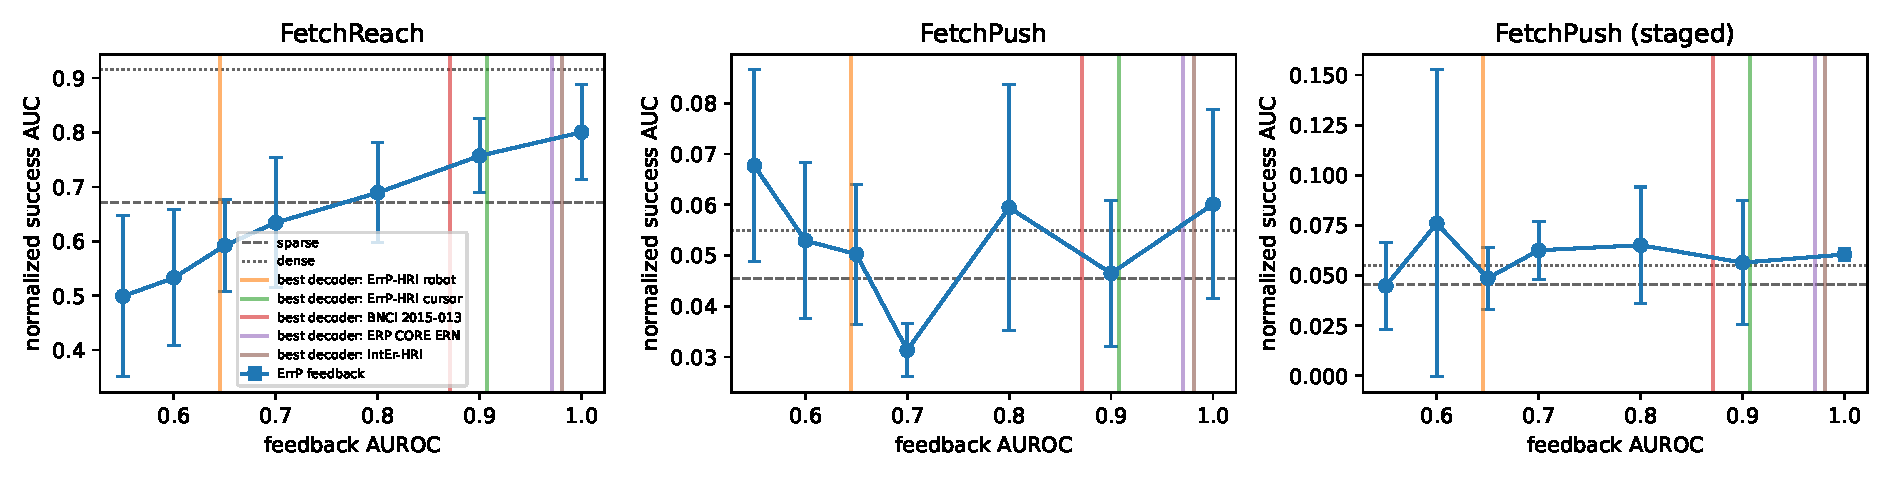
\includegraphics[width=\linewidth]{figures/frontier.pdf}
\caption{Decoder-quality frontier. Normalized success AUC (mean $\pm$ SD over five seeds) of SAC with ErrP
feedback of controlled AUROC; horizontal lines: sparse and dense reward. Vertical lines: the cross-subject AUROC
of the best ErrP-Bench decoder on each dataset.}
\label{fig:frontier}
\end{figure}

\begin{figure}[t]
\centering
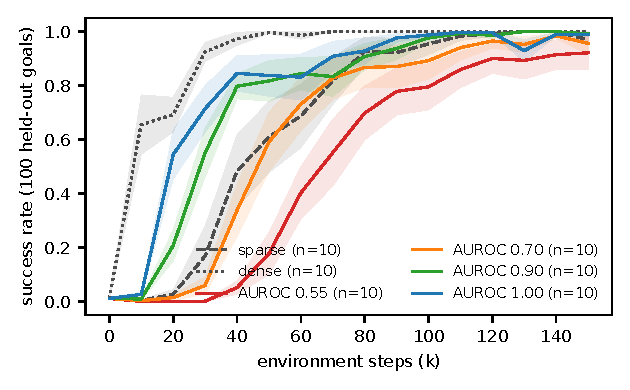
\includegraphics[width=0.62\linewidth]{figures/rl_curves.pdf}
\caption{FetchReach learning curves (success on 100 held-out goals; mean $\pm$ s.e.m. over 10 seeds) for sparse
and dense reward and for ErrP feedback of four quality levels. Low-quality feedback delays learning relative to
the sparse reward; high-quality feedback accelerates it.}
\label{fig:rlcurves}
\end{figure}

\begin{table}[t]
\centering
\caption{Normalized success AUC (mean $\pm$ SD over seeds) and its paired difference to the sparse-reward run of
the same seed ($k/n$: seeds with a positive difference).}
\label{tab:rl}
\scriptsize
\resizebox{\linewidth}{!}{\begin{tabular}{lcccccc}
\toprule
Feedback & \multicolumn{2}{c}{FetchReach} & \multicolumn{2}{c}{FetchPush} & \multicolumn{2}{c}{FetchPush (staged)} \\
 & norm.\ AUC & $\Delta$ vs sparse & norm.\ AUC & $\Delta$ vs sparse & norm.\ AUC & $\Delta$ vs sparse \\
\midrule
sparse only & 0.671\scriptsize{$\pm$0.106} & ref & 0.045\scriptsize{$\pm$0.011} & ref & 0.045\scriptsize{$\pm$0.011} & ref \\
dense (reference) & 0.915\scriptsize{$\pm$0.029} & +0.245 (10/10) & 0.055\scriptsize{$\pm$0.007} & +0.009 (5/5) & 0.053\scriptsize{$\pm$0.015} & +0.008 (4/5) \\
AUROC 0.55 & 0.499\scriptsize{$\pm$0.148} & -0.172 (1/10) & 0.068\scriptsize{$\pm$0.019} & +0.022 (4/5) & 0.045\scriptsize{$\pm$0.022} & -0.001 (2/5) \\
AUROC 0.60 & 0.533\scriptsize{$\pm$0.125} & -0.138 (2/10) & 0.053\scriptsize{$\pm$0.015} & +0.007 (4/5) & 0.076\scriptsize{$\pm$0.077} & +0.031 (3/5) \\
AUROC 0.65 & 0.592\scriptsize{$\pm$0.084} & -0.078 (1/10) & 0.050\scriptsize{$\pm$0.014} & +0.005 (4/5) & 0.049\scriptsize{$\pm$0.015} & +0.003 (3/5) \\
AUROC 0.70 & 0.634\scriptsize{$\pm$0.120} & -0.036 (5/10) & 0.031\scriptsize{$\pm$0.005} & -0.014 (0/5) & 0.063\scriptsize{$\pm$0.014} & +0.017 (5/5) \\
AUROC 0.80 & 0.689\scriptsize{$\pm$0.092} & +0.019 (5/10) & 0.059\scriptsize{$\pm$0.024} & +0.014 (4/5) & 0.065\scriptsize{$\pm$0.029} & +0.020 (4/5) \\
AUROC 0.90 & 0.757\scriptsize{$\pm$0.068} & +0.087 (6/10) & 0.046\scriptsize{$\pm$0.014} & +0.001 (2/5) & 0.056\scriptsize{$\pm$0.031} & +0.011 (3/5) \\
AUROC 1.00 (exact) & 0.800\scriptsize{$\pm$0.087} & +0.130 (9/10) & 0.060\scriptsize{$\pm$0.019} & +0.015 (4/5) & 0.061\scriptsize{$\pm$0.003} & +0.015 (4/5) \\
\bottomrule
\end{tabular}
}
\end{table}
